\section{Laboratory work implementation}

\subsection{Tasks and Points}

- Realizeaza o aplicatie care va implimenta tehnica Pomodoro SAU\\
\indent 
- O alta aplicatie sofisticata la alegere (Game) 

\subsection{Analiza lucrarii de laborator}
\selectlanguage{russian}
В ходе данной лабораторной работы было создано приложение Pomodoro, позволяющее правильно распределять собственное время. Логика работы данного приложения заключается в том, что каждый промежуток времени срабатывается таймер. Присутствует два вида времени: рабочее время и время отдыха. Таймер чередует два этих времени.\\
\indent 
Программа создана на Java, используя IDE AndroidStudio. Эммуляция программы производилась через эммулятор Genymotion. Программа работает и в фоновом режиме.\\
\indent 
Разработанная программа состоит из одного Activity и Service. Сервис позволяет работать в фоновом режиме. Окно содержит такие элементы, как textview, edittext, button. Время в минутах вводится в два edittext. После нажатия на кнопку Start, запускается сервис с таймером. Каждую секунду отсчитывается оставшееся время и выводится на экран. По завершению интервала звучит мелодия и появляется диалоговое окно с информацией. При закрытии окна, запускается таймер со вторым временем. При нажатии на кнопку Cancel таймер останавливается и удаляется сервис. Сервис представляет собой ни что иное, как отдельный процесс, в котором выполняется отдельная логика. \\
\indent 
Коды можно просмотреть на репозитории 



\subsection{Imagini}

\begin{figure}[h]
	\center{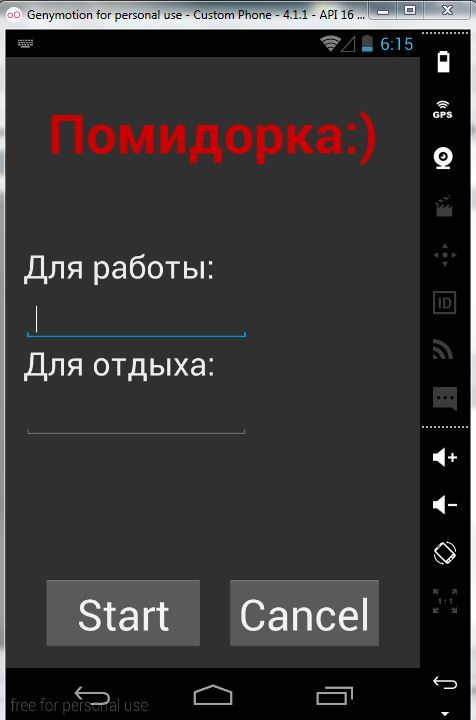
\includegraphics[width=0.3\linewidth]{images/DB.jpg}}
	\caption{Окно приложения}
	\label{ris:image}
\end{figure}
\hfill
\begin{figure}[h]
	\center{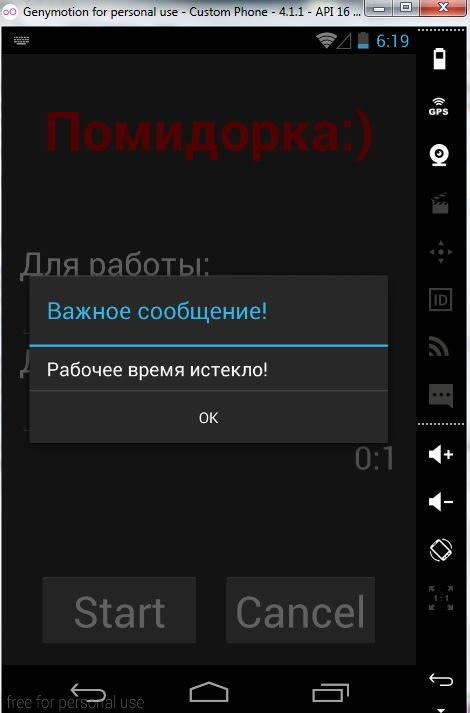
\includegraphics[width=0.3\linewidth]{images/Regestr.jpg}}
	\caption{Диалоговое окно}
	\label{ris:image}
\end{figure}

\clearpage